% Options for packages loaded elsewhere
% Options for packages loaded elsewhere
\PassOptionsToPackage{unicode}{hyperref}
\PassOptionsToPackage{hyphens}{url}
\PassOptionsToPackage{dvipsnames,svgnames,x11names}{xcolor}
%
\documentclass[
  spanish,
  us-letterpaper,
  DIV=11,
  numbers=noendperiod]{scrreprt}
\usepackage{xcolor}
\usepackage{amsmath,amssymb}
\setcounter{secnumdepth}{5}
\usepackage{iftex}
\ifPDFTeX
  \usepackage[T1]{fontenc}
  \usepackage[utf8]{inputenc}
  \usepackage{textcomp} % provide euro and other symbols
\else % if luatex or xetex
  \usepackage{unicode-math} % this also loads fontspec
  \defaultfontfeatures{Scale=MatchLowercase}
  \defaultfontfeatures[\rmfamily]{Ligatures=TeX,Scale=1}
\fi
\usepackage{lmodern}
\ifPDFTeX\else
  % xetex/luatex font selection
\fi
% Use upquote if available, for straight quotes in verbatim environments
\IfFileExists{upquote.sty}{\usepackage{upquote}}{}
\IfFileExists{microtype.sty}{% use microtype if available
  \usepackage[]{microtype}
  \UseMicrotypeSet[protrusion]{basicmath} % disable protrusion for tt fonts
}{}
\makeatletter
\@ifundefined{KOMAClassName}{% if non-KOMA class
  \IfFileExists{parskip.sty}{%
    \usepackage{parskip}
  }{% else
    \setlength{\parindent}{0pt}
    \setlength{\parskip}{6pt plus 2pt minus 1pt}}
}{% if KOMA class
  \KOMAoptions{parskip=half}}
\makeatother
% Make \paragraph and \subparagraph free-standing
\makeatletter
\ifx\paragraph\undefined\else
  \let\oldparagraph\paragraph
  \renewcommand{\paragraph}{
    \@ifstar
      \xxxParagraphStar
      \xxxParagraphNoStar
  }
  \newcommand{\xxxParagraphStar}[1]{\oldparagraph*{#1}\mbox{}}
  \newcommand{\xxxParagraphNoStar}[1]{\oldparagraph{#1}\mbox{}}
\fi
\ifx\subparagraph\undefined\else
  \let\oldsubparagraph\subparagraph
  \renewcommand{\subparagraph}{
    \@ifstar
      \xxxSubParagraphStar
      \xxxSubParagraphNoStar
  }
  \newcommand{\xxxSubParagraphStar}[1]{\oldsubparagraph*{#1}\mbox{}}
  \newcommand{\xxxSubParagraphNoStar}[1]{\oldsubparagraph{#1}\mbox{}}
\fi
\makeatother

\usepackage{color}
\usepackage{fancyvrb}
\newcommand{\VerbBar}{|}
\newcommand{\VERB}{\Verb[commandchars=\\\{\}]}
\DefineVerbatimEnvironment{Highlighting}{Verbatim}{commandchars=\\\{\}}
% Add ',fontsize=\small' for more characters per line
\usepackage{framed}
\definecolor{shadecolor}{RGB}{241,243,245}
\newenvironment{Shaded}{\begin{snugshade}}{\end{snugshade}}
\newcommand{\AlertTok}[1]{\textcolor[rgb]{0.68,0.00,0.00}{#1}}
\newcommand{\AnnotationTok}[1]{\textcolor[rgb]{0.37,0.37,0.37}{#1}}
\newcommand{\AttributeTok}[1]{\textcolor[rgb]{0.40,0.45,0.13}{#1}}
\newcommand{\BaseNTok}[1]{\textcolor[rgb]{0.68,0.00,0.00}{#1}}
\newcommand{\BuiltInTok}[1]{\textcolor[rgb]{0.00,0.23,0.31}{#1}}
\newcommand{\CharTok}[1]{\textcolor[rgb]{0.13,0.47,0.30}{#1}}
\newcommand{\CommentTok}[1]{\textcolor[rgb]{0.37,0.37,0.37}{#1}}
\newcommand{\CommentVarTok}[1]{\textcolor[rgb]{0.37,0.37,0.37}{\textit{#1}}}
\newcommand{\ConstantTok}[1]{\textcolor[rgb]{0.56,0.35,0.01}{#1}}
\newcommand{\ControlFlowTok}[1]{\textcolor[rgb]{0.00,0.23,0.31}{\textbf{#1}}}
\newcommand{\DataTypeTok}[1]{\textcolor[rgb]{0.68,0.00,0.00}{#1}}
\newcommand{\DecValTok}[1]{\textcolor[rgb]{0.68,0.00,0.00}{#1}}
\newcommand{\DocumentationTok}[1]{\textcolor[rgb]{0.37,0.37,0.37}{\textit{#1}}}
\newcommand{\ErrorTok}[1]{\textcolor[rgb]{0.68,0.00,0.00}{#1}}
\newcommand{\ExtensionTok}[1]{\textcolor[rgb]{0.00,0.23,0.31}{#1}}
\newcommand{\FloatTok}[1]{\textcolor[rgb]{0.68,0.00,0.00}{#1}}
\newcommand{\FunctionTok}[1]{\textcolor[rgb]{0.28,0.35,0.67}{#1}}
\newcommand{\ImportTok}[1]{\textcolor[rgb]{0.00,0.46,0.62}{#1}}
\newcommand{\InformationTok}[1]{\textcolor[rgb]{0.37,0.37,0.37}{#1}}
\newcommand{\KeywordTok}[1]{\textcolor[rgb]{0.00,0.23,0.31}{\textbf{#1}}}
\newcommand{\NormalTok}[1]{\textcolor[rgb]{0.00,0.23,0.31}{#1}}
\newcommand{\OperatorTok}[1]{\textcolor[rgb]{0.37,0.37,0.37}{#1}}
\newcommand{\OtherTok}[1]{\textcolor[rgb]{0.00,0.23,0.31}{#1}}
\newcommand{\PreprocessorTok}[1]{\textcolor[rgb]{0.68,0.00,0.00}{#1}}
\newcommand{\RegionMarkerTok}[1]{\textcolor[rgb]{0.00,0.23,0.31}{#1}}
\newcommand{\SpecialCharTok}[1]{\textcolor[rgb]{0.37,0.37,0.37}{#1}}
\newcommand{\SpecialStringTok}[1]{\textcolor[rgb]{0.13,0.47,0.30}{#1}}
\newcommand{\StringTok}[1]{\textcolor[rgb]{0.13,0.47,0.30}{#1}}
\newcommand{\VariableTok}[1]{\textcolor[rgb]{0.07,0.07,0.07}{#1}}
\newcommand{\VerbatimStringTok}[1]{\textcolor[rgb]{0.13,0.47,0.30}{#1}}
\newcommand{\WarningTok}[1]{\textcolor[rgb]{0.37,0.37,0.37}{\textit{#1}}}

\usepackage{longtable,booktabs,array}
\usepackage{calc} % for calculating minipage widths
% Correct order of tables after \paragraph or \subparagraph
\usepackage{etoolbox}
\makeatletter
\patchcmd\longtable{\par}{\if@noskipsec\mbox{}\fi\par}{}{}
\makeatother
% Allow footnotes in longtable head/foot
\IfFileExists{footnotehyper.sty}{\usepackage{footnotehyper}}{\usepackage{footnote}}
\makesavenoteenv{longtable}
\usepackage{graphicx}
\makeatletter
\newsavebox\pandoc@box
\newcommand*\pandocbounded[1]{% scales image to fit in text height/width
  \sbox\pandoc@box{#1}%
  \Gscale@div\@tempa{\textheight}{\dimexpr\ht\pandoc@box+\dp\pandoc@box\relax}%
  \Gscale@div\@tempb{\linewidth}{\wd\pandoc@box}%
  \ifdim\@tempb\p@<\@tempa\p@\let\@tempa\@tempb\fi% select the smaller of both
  \ifdim\@tempa\p@<\p@\scalebox{\@tempa}{\usebox\pandoc@box}%
  \else\usebox{\pandoc@box}%
  \fi%
}
% Set default figure placement to htbp
\def\fps@figure{htbp}
\makeatother


% definitions for citeproc citations
\NewDocumentCommand\citeproctext{}{}
\NewDocumentCommand\citeproc{mm}{%
  \begingroup\def\citeproctext{#2}\cite{#1}\endgroup}
\makeatletter
 % allow citations to break across lines
 \let\@cite@ofmt\@firstofone
 % avoid brackets around text for \cite:
 \def\@biblabel#1{}
 \def\@cite#1#2{{#1\if@tempswa , #2\fi}}
\makeatother
\newlength{\cslhangindent}
\setlength{\cslhangindent}{1.5em}
\newlength{\csllabelwidth}
\setlength{\csllabelwidth}{3em}
\newenvironment{CSLReferences}[2] % #1 hanging-indent, #2 entry-spacing
 {\begin{list}{}{%
  \setlength{\itemindent}{0pt}
  \setlength{\leftmargin}{0pt}
  \setlength{\parsep}{0pt}
  % turn on hanging indent if param 1 is 1
  \ifodd #1
   \setlength{\leftmargin}{\cslhangindent}
   \setlength{\itemindent}{-1\cslhangindent}
  \fi
  % set entry spacing
  \setlength{\itemsep}{#2\baselineskip}}}
 {\end{list}}
\usepackage{calc}
\newcommand{\CSLBlock}[1]{\hfill\break\parbox[t]{\linewidth}{\strut\ignorespaces#1\strut}}
\newcommand{\CSLLeftMargin}[1]{\parbox[t]{\csllabelwidth}{\strut#1\strut}}
\newcommand{\CSLRightInline}[1]{\parbox[t]{\linewidth - \csllabelwidth}{\strut#1\strut}}
\newcommand{\CSLIndent}[1]{\hspace{\cslhangindent}#1}

\ifLuaTeX
\usepackage[bidi=basic]{babel}
\else
\usepackage[bidi=default]{babel}
\fi
% get rid of language-specific shorthands (see #6817):
\let\LanguageShortHands\languageshorthands
\def\languageshorthands#1{}


\setlength{\emergencystretch}{3em} % prevent overfull lines

\providecommand{\tightlist}{%
  \setlength{\itemsep}{0pt}\setlength{\parskip}{0pt}}



 


\KOMAoption{captions}{tableheading}
\makeatletter
\@ifpackageloaded{bookmark}{}{\usepackage{bookmark}}
\makeatother
\makeatletter
\@ifpackageloaded{caption}{}{\usepackage{caption}}
\AtBeginDocument{%
\ifdefined\contentsname
  \renewcommand*\contentsname{Tabla de contenidos}
\else
  \newcommand\contentsname{Tabla de contenidos}
\fi
\ifdefined\listfigurename
  \renewcommand*\listfigurename{Listado de Figuras}
\else
  \newcommand\listfigurename{Listado de Figuras}
\fi
\ifdefined\listtablename
  \renewcommand*\listtablename{Listado de Tablas}
\else
  \newcommand\listtablename{Listado de Tablas}
\fi
\ifdefined\figurename
  \renewcommand*\figurename{Figura}
\else
  \newcommand\figurename{Figura}
\fi
\ifdefined\tablename
  \renewcommand*\tablename{Tabla}
\else
  \newcommand\tablename{Tabla}
\fi
}
\@ifpackageloaded{float}{}{\usepackage{float}}
\floatstyle{ruled}
\@ifundefined{c@chapter}{\newfloat{codelisting}{h}{lop}}{\newfloat{codelisting}{h}{lop}[chapter]}
\floatname{codelisting}{Listado}
\newcommand*\listoflistings{\listof{codelisting}{Listado de Listados}}
\makeatother
\makeatletter
\makeatother
\makeatletter
\@ifpackageloaded{caption}{}{\usepackage{caption}}
\@ifpackageloaded{subcaption}{}{\usepackage{subcaption}}
\makeatother
\usepackage{bookmark}
\IfFileExists{xurl.sty}{\usepackage{xurl}}{} % add URL line breaks if available
\urlstyle{same}
\hypersetup{
  pdftitle={Estimación de la temperatura con la ecuacion del Bio-Calor usando DeepONet},
  pdfauthor={Francisco Damián Escobar Candelaria; Yofre Hernán García Gómez},
  pdflang={es},
  colorlinks=true,
  linkcolor={blue},
  filecolor={Maroon},
  citecolor={Blue},
  urlcolor={Blue},
  pdfcreator={LaTeX via pandoc}}


\title{Estimación de la temperatura con la ecuacion del Bio-Calor usando
DeepONet}
\author{Francisco Damián Escobar Candelaria \and Yofre Hernán García
Gómez}
\date{2025-04-21}
\begin{document}
\maketitle

\renewcommand*\contentsname{Tabla de contenidos}
{
\hypersetup{linkcolor=}
\setcounter{tocdepth}{2}
\tableofcontents
}

\bookmarksetup{startatroot}

\chapter*{Resumen}\label{resumen}
\addcontentsline{toc}{chapter}{Resumen}

\markboth{Resumen}{Resumen}

Aquí irá el resumen de la tesis.

\bookmarksetup{startatroot}

\chapter{Introducción}\label{introducciuxf3n}

\part{Redes neuronales}

\chapter{Physic Informed Neural Networks
(PINNs)}\label{physic-informed-neural-networks-pinns}

Las Physics-Informed Neural Networks (PINNs) son un enfoque innovador
que combina redes neuronales con ecuaciones diferenciales gobernantes
para resolver problemas complejos de física
(\citeproc{ref-blechs2021}{Blechschmidt y Ernst 2021}). A diferencia de
métodos tradicionales, las PINNs incorporan directamente las ecuaciones
físicas en su función de pérdida mediante diferenciación automática, lo
que permite minimizar simultáneamente el error en los datos y el
residual de las PDEs (\citeproc{ref-karniadakis2021}{Karniadakis et~al.
2021}). Esta característica las hace particularmente valiosas en
escenarios con datos limitados, donde el conocimiento físico actúa como
un regularizador efectivo . La capacidad de aproximación de las PINNs se
fundamenta en el teorema de aproximación universal de las redes
neuronales, adaptado para incorporar restricciones físicas a través de
términos de penalización en la función de optimización
(\citeproc{ref-karniadakis2021}{Karniadakis et~al. 2021}).

\section{Comparación con Redes Neuronales
Tradicionales}\label{comparaciuxf3n-con-redes-neuronales-tradicionales}

Mientras que las redes neuronales tradicionales dependen exclusivamente
de grandes volúmenes de datos etiquetados para su entrenamiento
(\citeproc{ref-karniadakis2021}{Karniadakis et~al. 2021}), las PINNs
integran el conocimiento físico como parte esencial de su arquitectura
(\citeproc{ref-blechs2021}{Blechschmidt y Ernst 2021}). Esta diferencia
clave permite a las PINNs generar soluciones físicamente consistentes
incluso con datos escasos, evitando el sobreajuste común en enfoques
puramente basados en datos. Otra ventaja significativa de las PINNs es
su naturaleza mesh-free, que contrasta con los métodos numéricos
tradicionales como FEM o FDM que requieren discretización espacial. Sin
embargo, el entrenamiento de PINNs puede ser más desafiante debido a la
necesidad de optimizar múltiples objetivos simultáneamente (ajuste a
datos y cumplimiento de leyes físicas)
(\citeproc{ref-blechs2021}{Blechschmidt y Ernst 2021};
\citeproc{ref-karniadakis2021}{Karniadakis et~al. 2021}).

\chapter{DeepONet}\label{deeponet}

\textbf{DeepONet} (Deep Operator Network) es una arquitectura de red
neuronal profunda diseñada para aprender operadores no lineales que
mapean funciones de entrada a funciones de salida. A diferencia de las
redes convencionales que aprenden funciones escalares, DeepONet se
enfoca en representar operadores completos, como soluciones de
ecuaciones diferenciales, a partir de datos observados o simulaciones
numérica (\citeproc{ref-lu2021deeponet}{Lu, Jin, et~al. 2021}).

\section{Arquitectura}\label{arquitectura}

La arquitectura de DeepONet está compuesta por dos redes principales: la
red de \emph{branch} y la red de \emph{trunk}. La red \emph{branch}
procesa las evaluaciones discretas de la función de entrada (por
ejemplo, condiciones iniciales o de frontera), mientras que la red
\emph{trunk} recibe como entrada los puntos del dominio donde se desea
evaluar la función de salida. La salida final se obtiene mediante el
producto punto de los vectores generados por ambas redes, lo que permite
representar operadores complejos con alta generalización a nuevos datos
(\citeproc{ref-lu2021deeponet}{Lu, Jin, et~al. 2021}).

\begin{figure}

\centering{

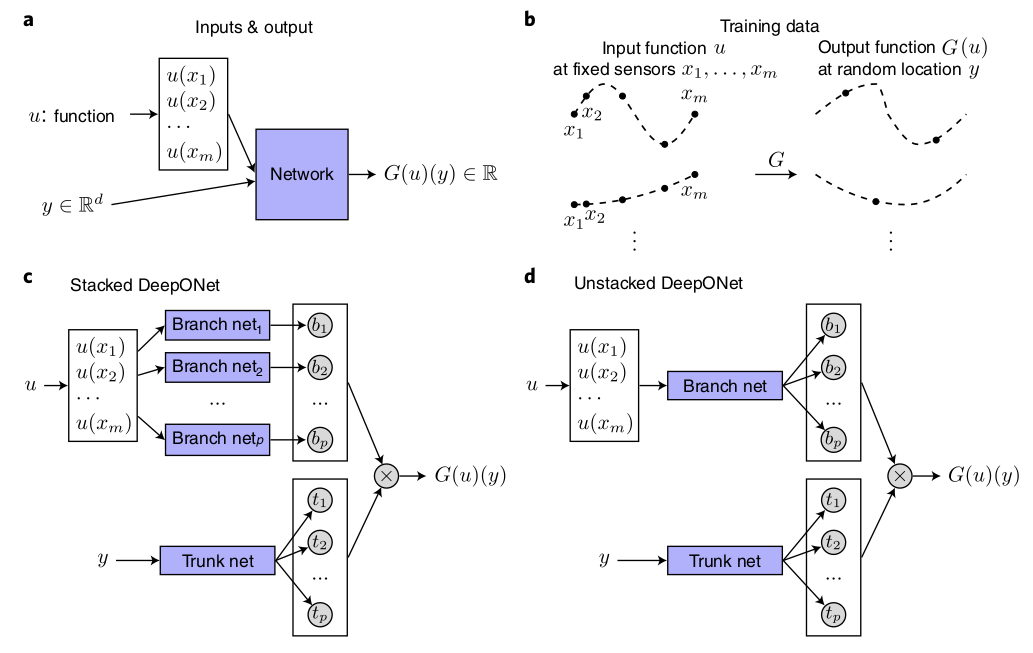
\includegraphics[width=6.25in,height=\textheight,keepaspectratio]{images/deeponet_architecture.png}

}

\caption{\label{fig-deeponet-arch}\textbf{Ilustraciones del
planteamiento del problema y arquitectura DeepONet que conducen a una
buena generalización. a)} Para que la red aprenda un operador
\(G : u \rightarrow G(u)\) se necesitan dos entradas
\([u(x_1), u(x_2), ..., u(x_m)]\) e \(y\). \textbf{b)} Ilustración de
los datos de entrenamiento. Para cada función de entrada \(u\), se
requiere el mismo número de evaluaciones en los mismos sensores
dispersos \(x_1, x_2, ..., x_m\). Sin embargo, no se impone ninguna
restricción sobre el número ni las ubicaciones para la evaluación de las
funciones de salida. \textbf{c)} La DeepONet \emph{stacked} se inspira
en el Teorema 1 y consta de una red \emph{Trunk} y \(p\) redes
\emph{Branch} apiladas. La red construida en el Teorema 1 es una
DeepONet \emph{stacked} formada al elegir la red \emph{Trunk} como una
red de una capa de ancho \(p\) y cada red \emph{Branch} como una red de
una capa oculta de ancho \(n\). \textbf{d)} La red DeepONet
\emph{unstacked} se inspira en el Teorema 2 y consta de una red
\emph{Trunk} y una red \emph{Branch}. Una red DeepONet \emph{unstacked}
puede considerarse como una red DeepONet \emph{stacked}, en la que todas
las redes \emph{Branch} comparten el mismo conjunto de parámetros
(\citeproc{ref-lu2021deeponet}{Lu, Jin, et~al. 2021}).}

\end{figure}%

\section{Comparación con una PINN}\label{comparaciuxf3n-con-una-pinn}

En contraste con una red PINN convencional (Physics-Informed Neural
Network), que resuelve una instancia específica de una ecuación
diferencial para un conjunto dado de condiciones, DeepONet aprende el
operador general que resuelve muchas instancias a la vez. Mientras que
una PINN debe ser reentrenada para cada nuevo problema, DeepONet, una
vez entrenado, puede predecir soluciones rápidamente para múltiples
condiciones nuevas. Esto lo hace especialmente eficiente en aplicaciones
donde se requiere realizar inferencias repetidas, como en control o
diseño inverso (\citeproc{ref-kumar2024deeponet}{Kumar et~al. 2024}).

\part{Ecuación del Bio-Calor}

La ecuación del bio-calor, formulada por Pennes
(\citeproc{ref-pennes1948}{1948}), surgió de su estudio pionero
\emph{``Analysis of Tissue and Arterial Blood Temperatures in the
Resting Human Forearm''}. Publicado en el \emph{Journal of Applied
Physiology}, este trabajo fue el primero en cuantificar la interacción
entre la temperatura arterial y tisular en humanos. Pennes combinó
principios termodinámicos con mediciones experimentales en el antebrazo,
estableciendo un modelo matemático que relacionaba el flujo sanguíneo,
la producción metabólica de calor y la conducción térmica en tejidos.

\begin{figure}

\centering{

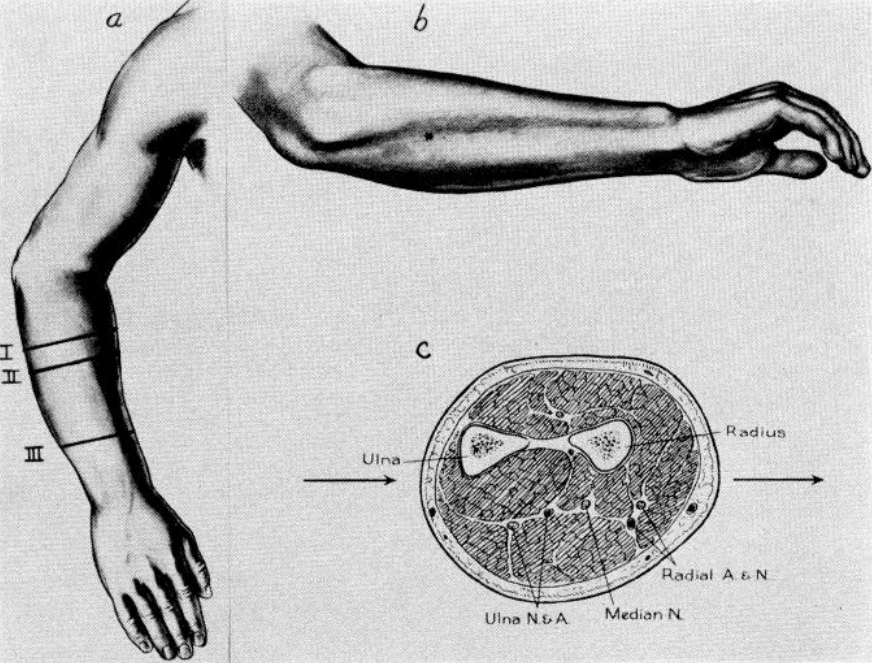
\includegraphics[width=5.20833in,height=\textheight,keepaspectratio]{images/pennes_art.png}

}

\caption{\label{fig-pennes_art}\textbf{a)} Posición del brazo derecho
(vista superior). La linea horizontal II indica el nivel de la figura
c). \textbf{b)} Posición del brazo derecho (vista lateral).
\textbf{c)}Sección transversal anatómica del antebrazo en el nivel II
(\citeproc{ref-pennes1948}{Pennes 1948}).}

\end{figure}%

El modelo de Pennes simplificó la complejidad biológica al asumir un
flujo sanguíneo uniforme y una transferencia de calor proporcional a la
diferencia entre la temperatura arterial y la tisular. Aunque
posteriores investigaciones refinaron sus supuestos, su ecuación sigue
siendo un referente en bioingeniería térmica. Su trabajo no solo sentó
las bases para aplicaciones clínicas, como la hipertermia oncológica,
sino que también inspiró avances en el estudio de la termorregulación
humana y el diseño de dispositivos médicos.

\chapter{Forma de la ecuación}\label{forma-de-la-ecuaciuxf3n}

La ecuación diferencial de bio-calor de Pennes
(\citeproc{ref-pennes1948}{1948}) modela la transferencia de calor en
tejidos biológicos, integrando efectos de conducción, perfusión
sanguínea y metabolismo. Su forma general es:

\begin{equation}\label{eq:PBHE_completa}
\rho c \frac{\partial T}{\partial t} = k_{\text{eff}} \frac{\partial^{2} T}{\partial x^{2}} - \rho_b c_b \omega_b (T - T_a) + Q, \quad x \in \Omega, \, t \in [0, t_f]
\end{equation}

\begin{longtable}[]{@{}lll@{}}
\toprule\noalign{}
Símbolo & Descripción & Unidades \\
\midrule\noalign{}
\endhead
\bottomrule\noalign{}
\endlastfoot
\(T\) & Temperatura del tejido & °C \\
\(\rho\) & Densidad del tejido & \(\dfrac{kg}{m^3}\) \\
\(c\) & Calor específico del tejido & \(\dfrac{J}{kg °C}\) \\
\(k_{\text{eff}}\) & Conductividad térmica & \(\dfrac{W}{m °C}\) \\
\(\rho_b\) & Densidad de la sangre & \(\dfrac{kg}{m^3}\) \\
\(c_b\) & Calor específico de la sangre & \(\dfrac{J}{kg °C}\) \\
\(\omega_b\) & Tasa de perfusión sanguínea & \(1/s\) \\
\(T_a\) & Temperatura arterial & °C \\
\(Q = q_m + q_p\) & Fuente de calor & \(\dfrac{W}{m^3}\) \\
\(q_m\) & Metabolismo & \(\dfrac{W}{m^3}\) \\
\(q_p\) & Externa & \(\dfrac{W}{m^3}\) \\
\end{longtable}

\section{Versión reducida
(adimensionalizada)}\label{versiuxf3n-reducida-adimensionalizada}

Mediante escalamiento: \begin{equation}
T' = T - T_a \qquad \theta = \dfrac{T'}{T_M - T_a} \qquad X = \dfrac{x}{L_0} \qquad \tau = \dfrac{t}{t_f}
\end{equation}

\begin{longtable}[]{@{}lll@{}}
\toprule\noalign{}
Símbolo & Descripción & Unidades \\
\midrule\noalign{}
\endhead
\bottomrule\noalign{}
\endlastfoot
\(L_0\) & Longitud característica del dominio & \(m\) \\
\(t_f\) & Tiempo final de simulación & \(s\) \\
\end{longtable}

se obtiene:

\begin{equation}
\partial_{\tau} \theta = a_1 \partial_{XX} \theta - a_2 W \theta + a_3
\end{equation}

\textbf{Parámetros adimensionales}:\\
- \(a_1 = \frac{t_f}{\alpha L_0^2}\) (difusividad térmica
\(\alpha = \frac{k_{\text{eff}}}{\rho c}\)).\\
- \(a_2 = \frac{t_f c_b}{\rho c}\).\\
- \(a_3 = \frac{t_f Q}{\rho c (T_M - T_a)}\).\\
- \(W = \rho_b \omega_b\): Tasa volumétrica de perfusión (kg/m³·s).

\section{Condiciones de uso
adecuadas}\label{condiciones-de-uso-adecuadas}

\begin{enumerate}
\def\labelenumi{\arabic{enumi}.}
\tightlist
\item
  \textbf{Tejidos homogéneos}: Aproximación válida para regiones con
  propiedades térmicas uniformes.\\
\item
  \textbf{Perfusión sanguínea constante}: Supone flujo sanguíneo estable
  en el dominio.\\
\item
  \textbf{Aplicaciones clínicas}: Hipertermia, crioterapia y modelado
  térmico en terapias oncológicas.
\end{enumerate}

\chapter{Modelado del Bio-Calor en
Hipertermia}\label{modelado-del-bio-calor-en-hipertermia}

La ecuación del bio-calor, formulada por Pennes
(\citeproc{ref-pennes1948}{1948}), permite modelar la distribución de
temperatura en tejidos biológicos considerando el flujo sanguíneo, la
conductividad térmica y fuentes internas o externas de calor. Su
modelación es fundamental en la física médica para predecir el
comportamiento térmico durante tratamientos como la hipertermia. Además,
constituye una herramienta poderosa en el desarrollo de simulaciones
computacionales aplicadas al diseño y control de terapias térmicas en
tejidos vivos.

\section{Aplicaciones recientes de la ecuación del
bio-calor}\label{aplicaciones-recientes-de-la-ecuaciuxf3n-del-bio-calor}

Quintero et~al. (\citeproc{ref-quintero2017}{2017}) desarrollan un
modelo basado en ecuaciones diferenciales parciales que integra la
ecuación del bio-calor y la ley de Arrhenius para estimar el daño
térmico en tratamientos de hipertermia superficial. Utilizan el método
de líneas para resolver el sistema y plantean un problema de
optimización que busca maximizar el daño al tejido tumoral minimizando
el daño colateral. Su trabajo demuestra cómo la modelación matemática
puede guiar estrategias terapéuticas más seguras y eficaces.

Dutta y Rangarajan (\citeproc{ref-dutta2018}{2018}) presentan una
solución analítica cerrada en dos dimensiones para la ecuación del
bio-calor, considerando modelos de conducción tanto de tipo Fourier como
no-Fourier. Mediante el uso de la transformada de Laplace, analizan la
influencia de parámetros fisiológicos como la perfusión sanguínea y el
tiempo de relajación térmica sobre la evolución de la temperatura. Su
investigación aporta una base teórica sólida para comprender la
propagación térmica en tejidos vivos durante la hipertermia terapéutica.

Yang et~al. (\citeproc{ref-yang2014}{2014}) propone una estrategia
numérica para resolver problemas inversos de conducción térmica en
tejidos biológicos multicapa, utilizando un enfoque en diferencias
finitas y el concepto de tiempo futuro. El estudio se enfoca en predecir
las condiciones de frontera necesarias para generar distribuciones de
temperatura deseadas. La implementación de este método permite estimar
parámetros relevantes en tiempo real, lo cual resulta esencial para el
control térmico preciso en procedimientos médicos no invasivos como la
hipertermia localizada.

\part{Estudio de caso}

Hipertermia como opción terapéutica complementaria en el manejo de
cáncer

\hfill\break

La Organización Mundial de la Salud (\citeproc{ref-omscancer}{2022}) en
su página web define Cáncer como:

\emph{«Cáncer» es un término genérico utilizado para designar un amplio
grupo de enfermedades que pueden afectar a cualquier parte del
organismo; también se habla de «tumores malignos» o «neoplasias
malignas». Una característica definitoria del cáncer es la
multiplicación rápida de células anormales que se extienden más allá de
sus límites habituales y pueden invadir partes adyacentes del cuerpo o
propagarse a otros órganos, en un proceso que se denomina «metástasis».
La extensión de las metástasis es la principal causa de muerte por la
enfermedad.}

Por su parte Instituto Nacional del Cáncer
(\citeproc{ref-nci2021}{2021}) aporta lo siguiente:

\emph{Es posible que el cáncer comience en cualquier parte del cuerpo
humano, formado por billones de células. En condiciones normales, las
células humanas se forman y se multiplican (mediante un proceso que se
llama división celular) para formar células nuevas a medida que el
cuerpo las necesita. Cuando las células envejecen o se dañan, mueren y
las células nuevas las reemplazan.} \emph{A veces el proceso no sigue
este orden y las células anormales o células dañadas se forman y se
multiplican cuando no deberían. Estas células tal vez formen tumores,
que son bultos de tejido. Los tumores son cancerosos (malignos) o no
cancerosos (benignos).}

\begin{figure}

\centering{

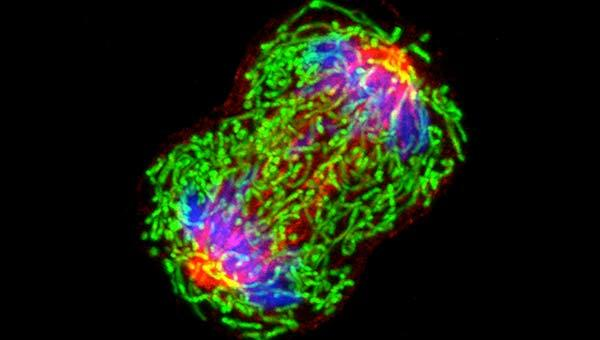
\includegraphics[width=5.20833in,height=\textheight,keepaspectratio]{images/dividing-breast-cancer-cell.jpg}

}

\caption{\label{fig-breast-cancer}Una célula de cáncer de seno que se
multiplica (\citeproc{ref-nci2021}{Instituto Nacional del Cáncer
2021}).}

\end{figure}%

Ésta enfermedad es la principal causa de muerte a nivel mundial, solo en
2020 arrebató casi 10 millones de vidas y según datos de Organización
Mundial de la Salud (\citeproc{ref-omscancer}{2022}) los cánceres más
comunes en 2020 fueron:

\begin{itemize}
\tightlist
\item
  De mama (2.26 millones de casos)
\item
  De pulmón (2.21 millones de casos)
\item
  De colon (1.93 millones de casos)
\item
  De próstata (1.41 millones de casos)
\item
  De piel (distinto del melanoma) (1.20 millones de casos)
\item
  Gástrico (1.09 millones de casos)
\end{itemize}

Es ante este panorama que distintos tratamientos surgen con el objetivo
de erradicar la enfermedad siempre que se tenga una detección oportuna.
Uno de dichos tratamientos es la hipertermia, según en el National
Cancer Institute (\citeproc{ref-hyperthermia}{2021}) es un método que
consiste en calentar el tejido corporal hasta los 39-45 °C para ayudar a
erradicar células cancerígenas con pequeñas o nulas lesiones en el
tejido sano. La hipertermia también es llamada terapia térmica o
termoterapia.

Uno de los principales retos de este tratamiento es la creación de un
modelo óptimo que se adecue al comportamiento de la transferencia de
calor que se hace a los tejidos con el fin de dañar únicamente el área
en el que se encuentran las célular cancerígenas, es por ello que los
modelos de integencia artificial y más precisamente las PINN's (aqui irá
una cita) surgen como posible solución a este reto.

El presente estudio utilizó como punto de partida el trabajo realizado
por Alessio Borgi (\citeproc{ref-medical_rep}{2023}) para modelar el
calentamiento del tejido corporal usando la ecuación del Bio-Calor en
dos dimensiones.

\chapter{Metodología}\label{metodologuxeda}

En esta sección se describe el enfoque metodológico utilizado para
evaluar la efectividad de una PINN utilizando una arquitectura DeepONet
con el objetivo de resolver la ecuacion del Bio-Calor. El proceso
metodológico se divide en las siguientes etapas:

\section{Aportaciones del modelo}\label{aportaciones-del-modelo}

Ya que se parte del trabajo de Alessio Borgi
(\citeproc{ref-medical_rep}{2023}), se examinó que dos de los puntos a
mejorar de la red neuronal que plantearon son:

\begin{enumerate}
\def\labelenumi{\arabic{enumi}.}
\tightlist
\item
  Desarrollar nuevas arquitecturas para la red neuronal y explorar
  nuevas configuraciones
\item
  Combinar las fortalezas de los algoritmos de optimización Adam y
  L-BFGS para mejorar la velocidad de convergencia y la precisión
\end{enumerate}

Tenindo los anteriores puntos en cuenta, se procedió a abordarlos e
implementarlos dentro del diseño del modelo.

\section{Diseño del modelo}\label{diseuxf1o-del-modelo}

El lenguaje seleccionado fué Python, a su vez el código se basa
enteramente en la librería Deepxde creada por Lu, Meng, et~al.
(\citeproc{ref-deepxde}{2021}) la cual está directamente enfocada a
resolver ecuaciones diferenciales, se usó además como backend
\emph{tensorflow\_compat\_v1} siendo su elección debida únicamente a la
familiarización previa que se tenía con ella. Finalmente el entorno
donde se programó y optimizó el código fué en \emph{Google Colab} ya que
la potencia de cómputo ofrecida por la plataforma era necesaria para
ejecutar el modelo.

\section{Implementación del modelo}\label{implementaciuxf3n-del-modelo}

Una vez creado el código que resuelve la ecuación del Bio-Calor, se
ajustaron los hiperparámetros tales como cantidad de épocas de
entrenamiento, el ratio de aprendizaje, la función de activación y el
inicializador en base al trabajo de Alessio Borgi
(\citeproc{ref-medical_rep}{2023}).

\section{Evaluación del modelo}\label{evaluaciuxf3n-del-modelo}

Se llevó a cabo una evaluación del modelo al darle como entrada un
conjunto de datos que no había visto y posteriormente obtener como
salida sus predicciones, con ellas se elaboraron gráficas claras y
detalladas de su pronóstico en el intervalo de tiempo y espacio
especificados.

\section{Comparación de resultados}\label{comparaciuxf3n-de-resultados}

Los resultados obtenidos de la evaluación del modelo fueron comparados
con los del trabajo de Alessio Borgi (\citeproc{ref-medical_rep}{2023})
para determinar su eficacia predictiva relativa. Se analizaron las
fortalezas y debilidades del modelo en función de su desempeño en la
predicción de las variables de interés.

\section{Análisis y conclusión}\label{anuxe1lisis-y-conclusiuxf3n}

Finalmente, se realizó un análisis detallado de los resultados obtenidos
para extraer conclusiones significativas. Se proporcionaron
recomendaciones basadas en los hallazgos del estudio, lo que permitió
establecer un marco para interpretaciones analíticas profundas y
recomendaciones bien fundamentadas en la sección de conclusiones del
estudio.

Este enfoque metodológico proporcionó una base sólida para los
resultados obtenidos, asegurando la integridad y la calidad del análisis
realizado en el estudio.

\chapter{Predicciones del modelo}\label{predicciones-del-modelo}

Conforme se ha referido previamente, se creó el modelo utilizando
Deepxde como base. Resulta relevante descatacar que se empleó la versión
1.10.1 de dicha librería. A continuación se presenta el código fuente de
la red neuronal

\begin{Shaded}
\begin{Highlighting}[]
\ImportTok{import}\NormalTok{ deepxde }\ImportTok{as}\NormalTok{ dde}
\ImportTok{import}\NormalTok{ numpy }\ImportTok{as}\NormalTok{ np}
\ImportTok{import}\NormalTok{ tensorflow }\ImportTok{as}\NormalTok{ tf}

\CommentTok{\# {-}{-}{-}{-}{-}{-}{-}{-}{-}{-}{-}{-}{-}{-}{-}{-}{-}{-}{-}{-}{-}{-}{-}{-}{-}{-}{-}{-}{-}{-}{-}{-}{-}{-}{-}{-}{-}{-}{-}{-}{-}{-}{-}{-}{-}{-}{-}{-}{-}{-}{-}{-}{-}{-}{-}{-}{-}{-}{-}{-}{-}{-}{-}{-}{-}{-}{-}{-}{-}{-}{-}{-}{-}{-}{-}{-}{-}{-}}
\CommentTok{\# Constants and Parameters}
\CommentTok{\# {-}{-}{-}{-}{-}{-}{-}{-}{-}{-}{-}{-}{-}{-}{-}{-}{-}{-}{-}{-}{-}{-}{-}{-}{-}{-}{-}{-}{-}{-}{-}{-}{-}{-}{-}{-}{-}{-}{-}{-}{-}{-}{-}{-}{-}{-}{-}{-}{-}{-}{-}{-}{-}{-}{-}{-}{-}{-}{-}{-}{-}{-}{-}{-}{-}{-}{-}{-}{-}{-}{-}{-}{-}{-}{-}{-}{-}{-}}

\CommentTok{\# Backend and seed}
\NormalTok{dde.backend.set\_default\_backend(}\StringTok{"tensorflow.compat.v1"}\NormalTok{)}
\NormalTok{dde.config.set\_random\_seed(}\DecValTok{123}\NormalTok{)}

\CommentTok{\# Physical parameters}
\NormalTok{heat\_coefficient }\OperatorTok{=} \FloatTok{1.0}
\NormalTok{p }\OperatorTok{=} \DecValTok{1050}
\NormalTok{c }\OperatorTok{=} \DecValTok{3639}
\NormalTok{keff }\OperatorTok{=} \DecValTok{5}
\NormalTok{tf }\OperatorTok{=} \DecValTok{1800}
\NormalTok{L0 }\OperatorTok{=} \FloatTok{0.05}
\NormalTok{cb }\OperatorTok{=} \DecValTok{3825}
\NormalTok{Q }\OperatorTok{=} \DecValTok{0}
\NormalTok{TM }\OperatorTok{=} \DecValTok{45}
\NormalTok{Ta }\OperatorTok{=} \DecValTok{37}
\NormalTok{alpha }\OperatorTok{=}\NormalTok{ p }\OperatorTok{*}\NormalTok{ c }\OperatorTok{/}\NormalTok{ keff}

\CommentTok{\# Dimensionless coefficients}
\NormalTok{a1 }\OperatorTok{=}\NormalTok{ tf }\OperatorTok{/}\NormalTok{ (alpha }\OperatorTok{*}\NormalTok{ L0}\OperatorTok{**}\DecValTok{2}\NormalTok{)}
\NormalTok{a2 }\OperatorTok{=}\NormalTok{ tf }\OperatorTok{*}\NormalTok{ cb }\OperatorTok{/}\NormalTok{ (p }\OperatorTok{*}\NormalTok{ c)}
\NormalTok{a3 }\OperatorTok{=}\NormalTok{ (tf }\OperatorTok{*}\NormalTok{ Q) }\OperatorTok{/}\NormalTok{ (p }\OperatorTok{*}\NormalTok{ c }\OperatorTok{*}\NormalTok{ (TM }\OperatorTok{{-}}\NormalTok{ Ta))}

\CommentTok{\# Domain boundaries}
\NormalTok{x\_initial, x\_boundary }\OperatorTok{=} \FloatTok{0.0}\NormalTok{, }\FloatTok{1.0}
\NormalTok{y\_initial, y\_boundary }\OperatorTok{=} \FloatTok{0.0}\NormalTok{, }\FloatTok{1.0}
\NormalTok{t\_initial, t\_final }\OperatorTok{=} \FloatTok{0.0}\NormalTok{, }\FloatTok{1.0}

\CommentTok{\# Dataset configuration}
\NormalTok{pts\_dom }\OperatorTok{=} \DecValTok{10}
\NormalTok{pts\_bc }\OperatorTok{=} \DecValTok{20}
\NormalTok{pts\_ic }\OperatorTok{=} \DecValTok{60}
\NormalTok{num\_test }\OperatorTok{=} \DecValTok{25}

\CommentTok{\# Sensor grid and function space}
\NormalTok{num\_sensors }\OperatorTok{=} \DecValTok{4}
\NormalTok{size\_cov\_matrix }\OperatorTok{=} \DecValTok{40}

\CommentTok{\# Network architecture}
\NormalTok{width\_net }\OperatorTok{=} \DecValTok{20}
\NormalTok{len\_net }\OperatorTok{=} \DecValTok{3}
\NormalTok{AF }\OperatorTok{=} \StringTok{"elu"}
\NormalTok{k\_initializer }\OperatorTok{=} \StringTok{"Glorot normal"}

\CommentTok{\# Training parameters}
\NormalTok{num\_iterations }\OperatorTok{=} \DecValTok{2000}
\NormalTok{learning\_rate }\OperatorTok{=} \FloatTok{2e{-}3}
\NormalTok{decay\_rate }\OperatorTok{=} \FloatTok{0.05}
\NormalTok{decay\_steps }\OperatorTok{=} \DecValTok{1000}

\CommentTok{\# {-}{-}{-}{-}{-}{-}{-}{-}{-}{-}{-}{-}{-}{-}{-}{-}{-}{-}{-}{-}{-}{-}{-}{-}{-}{-}{-}{-}{-}{-}{-}{-}{-}{-}{-}{-}{-}{-}{-}{-}{-}{-}{-}{-}{-}{-}{-}{-}{-}{-}{-}{-}{-}{-}{-}{-}{-}{-}{-}{-}{-}{-}{-}{-}{-}{-}{-}{-}{-}{-}{-}{-}{-}{-}{-}{-}{-}{-}}
\CommentTok{\# Geometry and Time Domain}
\CommentTok{\# {-}{-}{-}{-}{-}{-}{-}{-}{-}{-}{-}{-}{-}{-}{-}{-}{-}{-}{-}{-}{-}{-}{-}{-}{-}{-}{-}{-}{-}{-}{-}{-}{-}{-}{-}{-}{-}{-}{-}{-}{-}{-}{-}{-}{-}{-}{-}{-}{-}{-}{-}{-}{-}{-}{-}{-}{-}{-}{-}{-}{-}{-}{-}{-}{-}{-}{-}{-}{-}{-}{-}{-}{-}{-}{-}{-}{-}{-}}

\NormalTok{spatial\_domain }\OperatorTok{=}\NormalTok{ dde.geometry.Rectangle([x\_initial, y\_initial],}
\NormalTok{                                        [x\_boundary, y\_boundary])}
\NormalTok{time\_domain }\OperatorTok{=}\NormalTok{ dde.geometry.TimeDomain(t\_initial, t\_final)}
\NormalTok{geomtime }\OperatorTok{=}\NormalTok{ dde.geometry.GeometryXTime(spatial\_domain, time\_domain)}

\CommentTok{\# {-}{-}{-}{-}{-}{-}{-}{-}{-}{-}{-}{-}{-}{-}{-}{-}{-}{-}{-}{-}{-}{-}{-}{-}{-}{-}{-}{-}{-}{-}{-}{-}{-}{-}{-}{-}{-}{-}{-}{-}{-}{-}{-}{-}{-}{-}{-}{-}{-}{-}{-}{-}{-}{-}{-}{-}{-}{-}{-}{-}{-}{-}{-}{-}{-}{-}{-}{-}{-}{-}{-}{-}{-}{-}{-}{-}{-}{-}}
\CommentTok{\# PDE and Conditions}
\CommentTok{\# {-}{-}{-}{-}{-}{-}{-}{-}{-}{-}{-}{-}{-}{-}{-}{-}{-}{-}{-}{-}{-}{-}{-}{-}{-}{-}{-}{-}{-}{-}{-}{-}{-}{-}{-}{-}{-}{-}{-}{-}{-}{-}{-}{-}{-}{-}{-}{-}{-}{-}{-}{-}{-}{-}{-}{-}{-}{-}{-}{-}{-}{-}{-}{-}{-}{-}{-}{-}{-}{-}{-}{-}{-}{-}{-}{-}{-}{-}}

\KeywordTok{def}\NormalTok{ initial\_condition(X):}
    \ControlFlowTok{return} \DecValTok{0}

\KeywordTok{def}\NormalTok{ heat\_equation(func, u, coords):}
\NormalTok{    u\_t }\OperatorTok{=}\NormalTok{ dde.grad.jacobian(u, func, i}\OperatorTok{=}\DecValTok{0}\NormalTok{, j}\OperatorTok{=}\DecValTok{2}\NormalTok{)}
\NormalTok{    u\_xx }\OperatorTok{=}\NormalTok{ dde.grad.hessian(u, func, i}\OperatorTok{=}\DecValTok{0}\NormalTok{, j}\OperatorTok{=}\DecValTok{0}\NormalTok{)}
\NormalTok{    u\_yy }\OperatorTok{=}\NormalTok{ dde.grad.hessian(u, func, i}\OperatorTok{=}\DecValTok{1}\NormalTok{, j}\OperatorTok{=}\DecValTok{1}\NormalTok{)}
    \ControlFlowTok{return}\NormalTok{ a1 }\OperatorTok{*}\NormalTok{ u\_t }\OperatorTok{{-}}\NormalTok{ (u\_xx }\OperatorTok{+}\NormalTok{ u\_yy) }\OperatorTok{+}\NormalTok{ a2 }\OperatorTok{*}\NormalTok{ u}

\KeywordTok{def}\NormalTok{ zero\_value(X):}
    \ControlFlowTok{return} \DecValTok{0}

\KeywordTok{def}\NormalTok{ time\_value(X):}
    \ControlFlowTok{return}\NormalTok{ X[:, }\DecValTok{2}\NormalTok{]}

\KeywordTok{def}\NormalTok{ is\_on\_vertex(x):}
\NormalTok{    vertices }\OperatorTok{=}\NormalTok{ np.array([[x\_initial, y\_initial],}
\NormalTok{                         [x\_boundary, y\_initial],}
\NormalTok{                         [x\_initial, y\_boundary],}
\NormalTok{                         [x\_boundary, y\_boundary]])}
    \ControlFlowTok{return} \BuiltInTok{any}\NormalTok{(np.allclose(x, v) }\ControlFlowTok{for}\NormalTok{ v }\KeywordTok{in}\NormalTok{ vertices)}

\KeywordTok{def}\NormalTok{ is\_initial(X, on\_initial):}
    \ControlFlowTok{return}\NormalTok{ on\_initial }\KeywordTok{and}\NormalTok{ np.isclose(X[}\DecValTok{2}\NormalTok{], t\_initial)}

\KeywordTok{def}\NormalTok{ left\_boundary(X, on\_boundary):}
\NormalTok{    spatial }\OperatorTok{=}\NormalTok{ X[}\DecValTok{0}\NormalTok{:}\DecValTok{2}\NormalTok{]}
\NormalTok{    t }\OperatorTok{=}\NormalTok{ X[}\DecValTok{2}\NormalTok{]}
    \ControlFlowTok{return}\NormalTok{ (}
\NormalTok{        on\_boundary }
        \KeywordTok{and}\NormalTok{ np.isclose(spatial[}\DecValTok{0}\NormalTok{], x\_initial) }
        \KeywordTok{and} \KeywordTok{not}\NormalTok{ np.isclose(t, t\_initial) }
        \KeywordTok{and} \KeywordTok{not}\NormalTok{ is\_on\_vertex(spatial)}
\NormalTok{    )}

\KeywordTok{def}\NormalTok{ right\_boundary(X, on\_boundary):}
\NormalTok{    spatial }\OperatorTok{=}\NormalTok{ X[}\DecValTok{0}\NormalTok{:}\DecValTok{2}\NormalTok{]}
\NormalTok{    t }\OperatorTok{=}\NormalTok{ X[}\DecValTok{2}\NormalTok{]}
    \ControlFlowTok{return}\NormalTok{ (}
\NormalTok{        on\_boundary }
        \KeywordTok{and}\NormalTok{ np.isclose(spatial[}\DecValTok{0}\NormalTok{], x\_boundary) }
        \KeywordTok{and} \KeywordTok{not}\NormalTok{ np.isclose(t, t\_initial) }
        \KeywordTok{and} \KeywordTok{not}\NormalTok{ is\_on\_vertex(spatial)}
\NormalTok{    )}

\KeywordTok{def}\NormalTok{ up\_low\_boundary(X, on\_boundary):}
\NormalTok{    spatial }\OperatorTok{=}\NormalTok{ X[}\DecValTok{0}\NormalTok{:}\DecValTok{2}\NormalTok{]}
\NormalTok{    t }\OperatorTok{=}\NormalTok{ X[}\DecValTok{2}\NormalTok{]}
    \ControlFlowTok{return}\NormalTok{ (on\_boundary }
    \KeywordTok{and}\NormalTok{ (np.isclose(spatial[}\DecValTok{1}\NormalTok{], y\_initial) }
    \KeywordTok{or}\NormalTok{ np.isclose(spatial[}\DecValTok{1}\NormalTok{], y\_boundary)) }
    \KeywordTok{and} \KeywordTok{not}\NormalTok{ np.isclose(t, t\_initial) }
    \KeywordTok{and} \KeywordTok{not}\NormalTok{ is\_on\_vertex(spatial)}
\NormalTok{    )}

\CommentTok{\# Initial and boundary conditions}
\NormalTok{ic }\OperatorTok{=}\NormalTok{ dde.icbc.IC(geomtime, initial\_condition, is\_initial)}
\NormalTok{left\_bc }\OperatorTok{=}\NormalTok{ dde.icbc.DirichletBC(geomtime, }
\NormalTok{                                zero\_value, left\_boundary)}
\NormalTok{right\_bc }\OperatorTok{=}\NormalTok{ dde.icbc.NeumannBC(geomtime,}
\NormalTok{                                time\_value, right\_boundary)}
\NormalTok{up\_low\_bc }\OperatorTok{=}\NormalTok{ dde.icbc.NeumannBC(geomtime, }
\NormalTok{                                zero\_value, up\_low\_boundary)}

\CommentTok{\# {-}{-}{-}{-}{-}{-}{-}{-}{-}{-}{-}{-}{-}{-}{-}{-}{-}{-}{-}{-}{-}{-}{-}{-}{-}{-}{-}{-}{-}{-}{-}{-}{-}{-}{-}{-}{-}{-}{-}{-}{-}{-}{-}{-}{-}{-}{-}{-}{-}{-}{-}{-}{-}{-}{-}{-}{-}{-}{-}{-}{-}{-}{-}{-}{-}{-}{-}{-}{-}{-}{-}{-}{-}{-}{-}{-}{-}{-}}
\CommentTok{\# Dataset Construction}
\CommentTok{\# {-}{-}{-}{-}{-}{-}{-}{-}{-}{-}{-}{-}{-}{-}{-}{-}{-}{-}{-}{-}{-}{-}{-}{-}{-}{-}{-}{-}{-}{-}{-}{-}{-}{-}{-}{-}{-}{-}{-}{-}{-}{-}{-}{-}{-}{-}{-}{-}{-}{-}{-}{-}{-}{-}{-}{-}{-}{-}{-}{-}{-}{-}{-}{-}{-}{-}{-}{-}{-}{-}{-}{-}{-}{-}{-}{-}{-}{-}}

\NormalTok{pde\_data }\OperatorTok{=}\NormalTok{ dde.data.TimePDE(}
\NormalTok{    geomtime,}
\NormalTok{    heat\_equation,}
\NormalTok{    [ic, left\_bc, right\_bc, up\_low\_bc],}
\NormalTok{    num\_domain}\OperatorTok{=}\NormalTok{pts\_dom,}
\NormalTok{    num\_boundary}\OperatorTok{=}\NormalTok{pts\_bc,}
\NormalTok{    num\_initial}\OperatorTok{=}\NormalTok{pts\_ic }
\NormalTok{)}

\CommentTok{\# {-}{-}{-}{-}{-}{-}{-}{-}{-}{-}{-}{-}{-}{-}{-}{-}{-}{-}{-}{-}{-}{-}{-}{-}{-}{-}{-}{-}{-}{-}{-}{-}{-}{-}{-}{-}{-}{-}{-}{-}{-}{-}{-}{-}{-}{-}{-}{-}{-}{-}{-}{-}{-}{-}{-}{-}{-}{-}{-}{-}{-}{-}{-}{-}{-}{-}{-}{-}{-}{-}{-}{-}{-}{-}{-}{-}{-}{-}}
\CommentTok{\# Sensor Points and Function Space}
\CommentTok{\# {-}{-}{-}{-}{-}{-}{-}{-}{-}{-}{-}{-}{-}{-}{-}{-}{-}{-}{-}{-}{-}{-}{-}{-}{-}{-}{-}{-}{-}{-}{-}{-}{-}{-}{-}{-}{-}{-}{-}{-}{-}{-}{-}{-}{-}{-}{-}{-}{-}{-}{-}{-}{-}{-}{-}{-}{-}{-}{-}{-}{-}{-}{-}{-}{-}{-}{-}{-}{-}{-}{-}{-}{-}{-}{-}{-}{-}{-}}

\NormalTok{side }\OperatorTok{=}\NormalTok{ np.linspace(x\_initial, x\_boundary, num\_sensors }\OperatorTok{+} \DecValTok{1}\NormalTok{)}
\NormalTok{x, y }\OperatorTok{=}\NormalTok{ np.meshgrid(side, side, indexing}\OperatorTok{=}\StringTok{\textquotesingle{}xy\textquotesingle{}}\NormalTok{)}
\NormalTok{sensor\_pts }\OperatorTok{=}\NormalTok{ np.stack([x.ravel(), y.ravel()], axis}\OperatorTok{=}\DecValTok{1}\NormalTok{)}

\NormalTok{fs }\OperatorTok{=}\NormalTok{ dde.data.function\_spaces.GRF2D(N}\OperatorTok{=}\NormalTok{size\_cov\_matrix, }
\NormalTok{                                    interp}\OperatorTok{=}\StringTok{"linear"}\NormalTok{)}

\NormalTok{data }\OperatorTok{=}\NormalTok{ dde.data.PDEOperatorCartesianProd(}
\NormalTok{    pde\_data,}
\NormalTok{    fs,}
\NormalTok{    sensor\_pts,}
\NormalTok{    num\_function}\OperatorTok{=}\NormalTok{(num\_sensors }\OperatorTok{+} \DecValTok{1}\NormalTok{)}\OperatorTok{**}\DecValTok{2}\NormalTok{,}
\NormalTok{    function\_variables}\OperatorTok{=}\NormalTok{[}\DecValTok{0}\NormalTok{, }\DecValTok{1}\NormalTok{],}
\NormalTok{    num\_test}\OperatorTok{=}\NormalTok{num\_test}
\NormalTok{)}

\CommentTok{\# {-}{-}{-}{-}{-}{-}{-}{-}{-}{-}{-}{-}{-}{-}{-}{-}{-}{-}{-}{-}{-}{-}{-}{-}{-}{-}{-}{-}{-}{-}{-}{-}{-}{-}{-}{-}{-}{-}{-}{-}{-}{-}{-}{-}{-}{-}{-}{-}{-}{-}{-}{-}{-}{-}{-}{-}{-}{-}{-}{-}{-}{-}{-}{-}{-}{-}{-}{-}{-}{-}{-}{-}{-}{-}{-}{-}{-}{-}}
\CommentTok{\# Network Definition}
\CommentTok{\# {-}{-}{-}{-}{-}{-}{-}{-}{-}{-}{-}{-}{-}{-}{-}{-}{-}{-}{-}{-}{-}{-}{-}{-}{-}{-}{-}{-}{-}{-}{-}{-}{-}{-}{-}{-}{-}{-}{-}{-}{-}{-}{-}{-}{-}{-}{-}{-}{-}{-}{-}{-}{-}{-}{-}{-}{-}{-}{-}{-}{-}{-}{-}{-}{-}{-}{-}{-}{-}{-}{-}{-}{-}{-}{-}{-}{-}{-}}

\NormalTok{branch\_layers }\OperatorTok{=}\NormalTok{ [(num\_sensors }\OperatorTok{+} \DecValTok{1}\NormalTok{)}\OperatorTok{**}\DecValTok{2}\NormalTok{] }\OperatorTok{+}\NormalTok{ len\_net }\OperatorTok{*}\NormalTok{ [width\_net]}
\NormalTok{trunk\_layers }\OperatorTok{=}\NormalTok{ [}\DecValTok{3}\NormalTok{] }\OperatorTok{+}\NormalTok{ len\_net }\OperatorTok{*}\NormalTok{ [width\_net]}

\NormalTok{net }\OperatorTok{=}\NormalTok{ dde.nn.DeepONetCartesianProd(}
\NormalTok{    branch\_layers,}
\NormalTok{    trunk\_layers,}
\NormalTok{    activation}\OperatorTok{=}\NormalTok{AF,}
\NormalTok{    kernel\_initializer}\OperatorTok{=}\NormalTok{k\_initializer}
\NormalTok{)}

\CommentTok{\# {-}{-}{-}{-}{-}{-}{-}{-}{-}{-}{-}{-}{-}{-}{-}{-}{-}{-}{-}{-}{-}{-}{-}{-}{-}{-}{-}{-}{-}{-}{-}{-}{-}{-}{-}{-}{-}{-}{-}{-}{-}{-}{-}{-}{-}{-}{-}{-}{-}{-}{-}{-}{-}{-}{-}{-}{-}{-}{-}{-}{-}{-}{-}{-}{-}{-}{-}{-}{-}{-}{-}{-}{-}{-}{-}{-}{-}{-}}
\CommentTok{\# Model Compilation and Training}
\CommentTok{\# {-}{-}{-}{-}{-}{-}{-}{-}{-}{-}{-}{-}{-}{-}{-}{-}{-}{-}{-}{-}{-}{-}{-}{-}{-}{-}{-}{-}{-}{-}{-}{-}{-}{-}{-}{-}{-}{-}{-}{-}{-}{-}{-}{-}{-}{-}{-}{-}{-}{-}{-}{-}{-}{-}{-}{-}{-}{-}{-}{-}{-}{-}{-}{-}{-}{-}{-}{-}{-}{-}{-}{-}{-}{-}{-}{-}{-}{-}}

\NormalTok{model }\OperatorTok{=}\NormalTok{ dde.Model(data, net)}
\NormalTok{model.}\BuiltInTok{compile}\NormalTok{(}\StringTok{"adam"}\NormalTok{, lr}\OperatorTok{=}\NormalTok{learning\_rate, decay}\OperatorTok{=}\NormalTok{(}\StringTok{"inverse time"}\NormalTok{, decay\_steps, decay\_rate))}
\NormalTok{losshistory, train\_state }\OperatorTok{=}\NormalTok{ model.train(iterations}\OperatorTok{=}\NormalTok{num\_iterations)}

\CommentTok{\# Fine{-}tuning with LBFGS optimizer}
\NormalTok{model.}\BuiltInTok{compile}\NormalTok{(}\StringTok{"L{-}BFGS"}\NormalTok{)}
\NormalTok{losshistory, train\_state }\OperatorTok{=}\NormalTok{ model.train()}
\end{Highlighting}
\end{Shaded}

\begin{verbatim}
2025-05-20 18:13:28.894698: I tensorflow/tsl/cuda/cudart_stub.cc:28] Could not find cuda drivers on your machine, GPU will not be used.
2025-05-20 18:13:29.128141: I tensorflow/tsl/cuda/cudart_stub.cc:28] Could not find cuda drivers on your machine, GPU will not be used.
2025-05-20 18:13:29.130347: I tensorflow/core/platform/cpu_feature_guard.cc:182] This TensorFlow binary is optimized to use available CPU instructions in performance-critical operations.
To enable the following instructions: AVX2 FMA, in other operations, rebuild TensorFlow with the appropriate compiler flags.
2025-05-20 18:13:30.116682: W tensorflow/compiler/tf2tensorrt/utils/py_utils.cc:38] TF-TRT Warning: Could not find TensorRT
Using backend: tensorflow.compat.v1
Other supported backends: tensorflow, pytorch, jax, paddle.
paddle supports more examples now and is recommended.
\end{verbatim}

\begin{verbatim}
WARNING:tensorflow:From /home/damian/.local/lib/python3.8/site-packages/tensorflow/python/compat/v2_compat.py:107: disable_resource_variables (from tensorflow.python.ops.variable_scope) is deprecated and will be removed in a future version.
Instructions for updating:
non-resource variables are not supported in the long term
Setting the default backend to "tensorflow.compat.v1". You can change it in the ~/.deepxde/config.json file or export the DDE_BACKEND environment variable. Valid options are: tensorflow.compat.v1, tensorflow, pytorch, jax, paddle (all lowercase)
Compiling model...
Building DeepONetCartesianProd...
'build' took 0.098436 s
\end{verbatim}

\begin{verbatim}
/home/damian/.local/lib/python3.8/site-packages/deepxde/nn/tensorflow_compat_v1/deeponet.py:549: UserWarning:

`tf.layers.dense` is deprecated and will be removed in a future version. Please use `tf.keras.layers.Dense` instead.

/home/damian/.local/lib/python3.8/site-packages/deepxde/nn/tensorflow_compat_v1/deeponet.py:556: UserWarning:

`tf.layers.dense` is deprecated and will be removed in a future version. Please use `tf.keras.layers.Dense` instead.

/home/damian/.local/lib/python3.8/site-packages/deepxde/nn/tensorflow_compat_v1/deeponet.py:570: UserWarning:

`tf.layers.dense` is deprecated and will be removed in a future version. Please use `tf.keras.layers.Dense` instead.
\end{verbatim}

\begin{verbatim}
'compile' took 15.037677 s
\end{verbatim}

\begin{verbatim}
2025-05-20 18:13:46.885013: I tensorflow/compiler/mlir/mlir_graph_optimization_pass.cc:375] MLIR V1 optimization pass is not enabled
\end{verbatim}

\begin{verbatim}
Training model...

Step      Train loss                                            Test loss                                             Test metric
0         [2.57e+00, 4.03e-01, 4.13e-01, 6.71e-01, 1.05e+00]    [1.57e+00, 1.57e-01, 3.45e-01, 5.19e-01, 3.07e-01]    []  
1000      [3.97e-03, 3.15e-03, 3.81e-04, 2.63e-02, 1.86e-04]    [6.39e-03, 3.24e-03, 9.14e-04, 2.74e-02, 4.08e-04]    []  
2000      [1.23e-03, 1.01e-03, 1.47e-04, 2.58e-02, 7.37e-05]    [4.01e-03, 1.03e-03, 6.52e-04, 2.66e-02, 1.18e-04]    []  

Best model at step 2000:
  train loss: 2.83e-02
  test loss: 3.24e-02
  test metric: []

'train' took 22.959966 s

Compiling model...
'compile' took 34.020894 s

Training model...

Step      Train loss                                            Test loss                                             Test metric
2000      [1.23e-03, 1.01e-03, 1.47e-04, 2.58e-02, 7.37e-05]    [4.01e-03, 1.03e-03, 6.52e-04, 2.66e-02, 1.18e-04]    []  
INFO:tensorflow:Optimization terminated with:
  Message: CONVERGENCE: REL_REDUCTION_OF_F_<=_FACTR*EPSMCH
  Objective function value: 0.028235
  Number of iterations: 4
  Number of functions evaluations: 41
2041      [1.21e-03, 1.01e-03, 1.11e-04, 2.58e-02, 7.36e-05]    [3.90e-03, 1.03e-03, 5.92e-04, 2.66e-02, 1.17e-04]    []  

Best model at step 2041:
  train loss: 2.82e-02
  test loss: 3.22e-02
  test metric: []

'train' took 11.552876 s
\end{verbatim}

El historial de perdida para el conjunto de entrenamiento es el
siguiente:

\begin{figure}

\centering{

\begin{Shaded}
\begin{Highlighting}[]
\ImportTok{import}\NormalTok{ plotly.graph\_objects }\ImportTok{as}\NormalTok{ go}

\CommentTok{\# Nombres de las componentes del loss}
\NormalTok{loss\_labels }\OperatorTok{=}\NormalTok{ [}
    \StringTok{"PDE residual loss"}\NormalTok{,}
    \StringTok{"Initial‐condition loss"}\NormalTok{,}
    \StringTok{"Left‐boundary (Dirichlet) loss"}\NormalTok{,}
    \StringTok{"Right‐boundary (Neumann) loss"}\NormalTok{,}
    \StringTok{"Top/Bottom‐boundary (Neumann) loss"}
\NormalTok{]}

\CommentTok{\# Extraer pasos y pérdida de entrenamiento}
\NormalTok{steps }\OperatorTok{=}\NormalTok{ losshistory.steps}
\NormalTok{train\_loss }\OperatorTok{=}\NormalTok{ np.array(losshistory.loss\_train)}

\CommentTok{\# Crear figura}
\NormalTok{fig }\OperatorTok{=}\NormalTok{ go.Figure()}

\ControlFlowTok{for}\NormalTok{ i }\KeywordTok{in} \BuiltInTok{range}\NormalTok{(train\_loss.shape[}\DecValTok{1}\NormalTok{]):}
\NormalTok{    fig.add\_trace(go.Scatter(}
\NormalTok{        x}\OperatorTok{=}\NormalTok{steps,}
\NormalTok{        y}\OperatorTok{=}\NormalTok{train\_loss[:, i],}
\NormalTok{        mode}\OperatorTok{=}\StringTok{\textquotesingle{}lines\textquotesingle{}}\NormalTok{,}
\NormalTok{        name}\OperatorTok{=}\NormalTok{loss\_labels[i]}
\NormalTok{    ))}

\NormalTok{fig.update\_layout(}
\NormalTok{    title}\OperatorTok{=}\StringTok{"Training Loss history"}\NormalTok{,}
\NormalTok{    xaxis}\OperatorTok{=}\BuiltInTok{dict}\NormalTok{(title}\OperatorTok{=}\StringTok{"Iteration"}\NormalTok{, tickformat}\OperatorTok{=}\StringTok{".1e"}\NormalTok{),}
\NormalTok{    yaxis}\OperatorTok{=}\BuiltInTok{dict}\NormalTok{(title}\OperatorTok{=}\StringTok{"Loss"}\NormalTok{, }\BuiltInTok{type}\OperatorTok{=}\StringTok{"log"}\NormalTok{, tickformat}\OperatorTok{=}\StringTok{".1e"}\NormalTok{),}
\NormalTok{    template}\OperatorTok{=}\StringTok{"plotly\_white"}\NormalTok{,}
\NormalTok{    legend}\OperatorTok{=}\BuiltInTok{dict}\NormalTok{(x}\OperatorTok{=}\FloatTok{0.99}\NormalTok{, y}\OperatorTok{=}\FloatTok{0.99}\NormalTok{),}
\NormalTok{    font}\OperatorTok{=}\BuiltInTok{dict}\NormalTok{(size}\OperatorTok{=}\DecValTok{14}\NormalTok{)}
\NormalTok{)}
\CommentTok{\# fig.show()}
\end{Highlighting}
\end{Shaded}

}

\caption{\label{fig-training_loss}}

\end{figure}%

\begin{figure}

\centering{

\pandocbounded{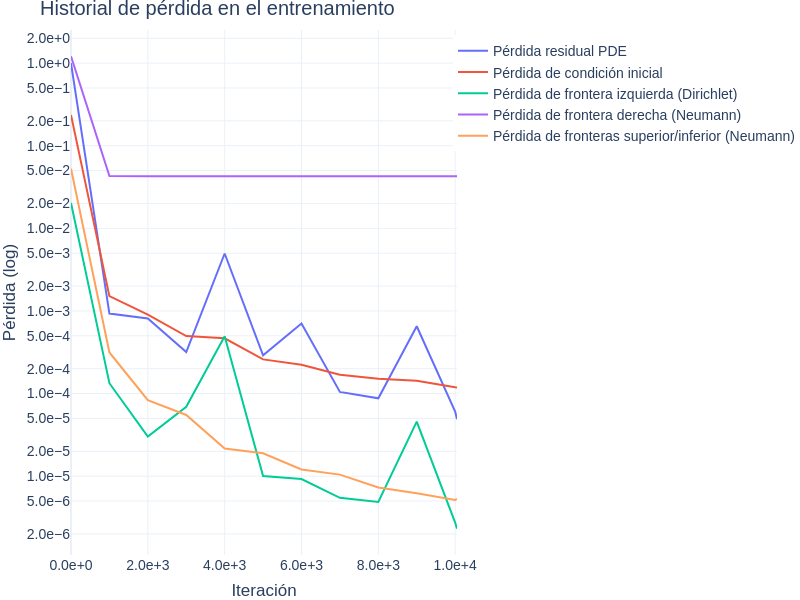
\includegraphics[keepaspectratio]{images/fig-training_loss.png}}

}

\caption{\label{fig-loss_training}Gráfica de la perdida en el
entrenamiento.}

\end{figure}%

El historial de perdida para el conjunto de prueba es el siguiente:

\begin{figure}

\centering{

\begin{Shaded}
\begin{Highlighting}[]
\ImportTok{import}\NormalTok{ plotly.graph\_objects }\ImportTok{as}\NormalTok{ go}

\CommentTok{\# Nombres de las componentes del loss}
\NormalTok{loss\_labels }\OperatorTok{=}\NormalTok{ [}
    \StringTok{"PDE residual loss"}\NormalTok{,}
    \StringTok{"Initial‐condition loss"}\NormalTok{,}
    \StringTok{"Left‐boundary (Dirichlet) loss"}\NormalTok{,}
    \StringTok{"Right‐boundary (Neumann) loss"}\NormalTok{,}
    \StringTok{"Top/Bottom‐boundary (Neumann) loss"}
\NormalTok{]}

\CommentTok{\# Extraer pasos y pérdida de entrenamiento}
\NormalTok{steps }\OperatorTok{=}\NormalTok{ losshistory.steps}
\NormalTok{test\_loss }\OperatorTok{=}\NormalTok{ np.array(losshistory.loss\_test)}

\CommentTok{\# Crear figura}
\NormalTok{fig }\OperatorTok{=}\NormalTok{ go.Figure()}

\ControlFlowTok{for}\NormalTok{ i }\KeywordTok{in} \BuiltInTok{range}\NormalTok{(test\_loss.shape[}\DecValTok{1}\NormalTok{]):}
\NormalTok{    fig.add\_trace(go.Scatter(}
\NormalTok{        x}\OperatorTok{=}\NormalTok{steps,}
\NormalTok{        y}\OperatorTok{=}\NormalTok{test\_loss[:, i],}
\NormalTok{        mode}\OperatorTok{=}\StringTok{\textquotesingle{}lines\textquotesingle{}}\NormalTok{,}
\NormalTok{        name}\OperatorTok{=}\NormalTok{loss\_labels[i]}
\NormalTok{    ))}

\NormalTok{fig.update\_layout(}
\NormalTok{    title}\OperatorTok{=}\StringTok{"Test Loss history"}\NormalTok{,}
\NormalTok{    xaxis}\OperatorTok{=}\BuiltInTok{dict}\NormalTok{(title}\OperatorTok{=}\StringTok{"Iteration"}\NormalTok{, tickformat}\OperatorTok{=}\StringTok{".1e"}\NormalTok{),}
\NormalTok{    yaxis}\OperatorTok{=}\BuiltInTok{dict}\NormalTok{(title}\OperatorTok{=}\StringTok{"Loss"}\NormalTok{, }\BuiltInTok{type}\OperatorTok{=}\StringTok{"log"}\NormalTok{, tickformat}\OperatorTok{=}\StringTok{".1e"}\NormalTok{),}
\NormalTok{    template}\OperatorTok{=}\StringTok{"plotly\_white"}\NormalTok{,}
\NormalTok{    legend}\OperatorTok{=}\BuiltInTok{dict}\NormalTok{(x}\OperatorTok{=}\FloatTok{0.99}\NormalTok{, y}\OperatorTok{=}\FloatTok{0.99}\NormalTok{),}
\NormalTok{    font}\OperatorTok{=}\BuiltInTok{dict}\NormalTok{(size}\OperatorTok{=}\DecValTok{14}\NormalTok{)}
\NormalTok{)}
\CommentTok{\# fig.show()}
\end{Highlighting}
\end{Shaded}

}

\caption{\label{fig-test_loss}}

\end{figure}%

\begin{figure}

\centering{

\pandocbounded{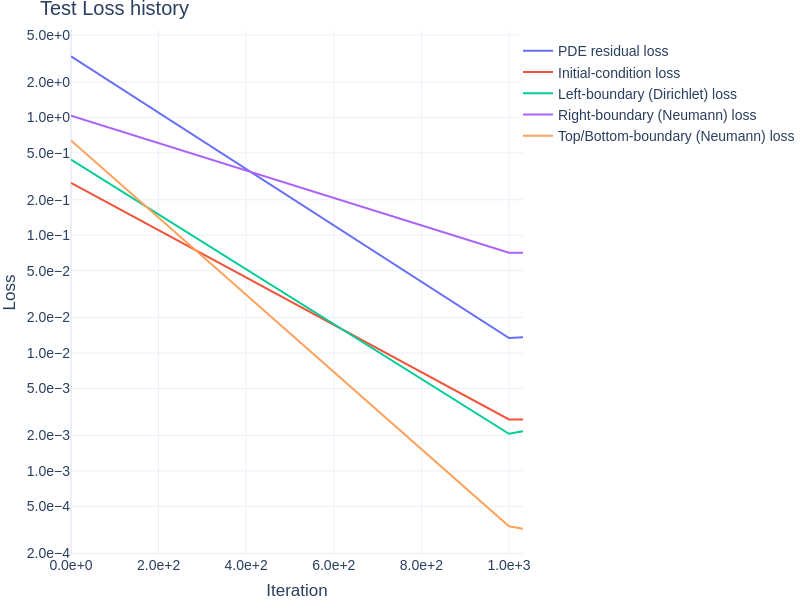
\includegraphics[keepaspectratio]{images/fig-test_loss.png}}

}

\caption{\label{fig-loss_test}Gráfica de la perdida en el conjunto de
prueba.}

\end{figure}%

A continuación, los valores predichos por la red neuronal a tiempos t(s)
de 0.0, 0.25, 0.50, 0.75 y 1.0.

\begin{Shaded}
\begin{Highlighting}[]
\ImportTok{import}\NormalTok{ matplotlib.pyplot }\ImportTok{as}\NormalTok{ plt}
\ImportTok{from}\NormalTok{ mpl\_toolkits.mplot3d }\ImportTok{import}\NormalTok{ Axes3D}
\ImportTok{import}\NormalTok{ matplotlib.gridspec }\ImportTok{as}\NormalTok{ gridspec}

\CommentTok{\# Times at which to evaluate the model}
\NormalTok{times }\OperatorTok{=}\NormalTok{ [}\FloatTok{0.0}\NormalTok{, }\FloatTok{0.25}\NormalTok{, }\FloatTok{0.5}\NormalTok{, }\FloatTok{0.75}\NormalTok{, }\FloatTok{1.0}\NormalTok{]}

\CommentTok{\# Generate a grid of (x, y) points}
\NormalTok{num\_points }\OperatorTok{=} \DecValTok{25}
\NormalTok{x }\OperatorTok{=}\NormalTok{ np.linspace(}\DecValTok{0}\NormalTok{, }\DecValTok{1}\NormalTok{, num\_points)}
\NormalTok{y }\OperatorTok{=}\NormalTok{ np.linspace(}\DecValTok{0}\NormalTok{, }\DecValTok{1}\NormalTok{, num\_points)}
\NormalTok{X, Y }\OperatorTok{=}\NormalTok{ np.meshgrid(x, y)}

\CommentTok{\# Create a figure and a GridSpec layout.}
\CommentTok{\# We reserve one row at the bottom for the colorbar.}
\NormalTok{ncols }\OperatorTok{=} \BuiltInTok{len}\NormalTok{(times)}
\NormalTok{fig }\OperatorTok{=}\NormalTok{ plt.figure(figsize}\OperatorTok{=}\NormalTok{((}\DecValTok{5} \OperatorTok{*}\NormalTok{ ncols) }\OperatorTok{+}\DecValTok{1}\NormalTok{, }\DecValTok{6}\NormalTok{))}
\NormalTok{gs }\OperatorTok{=}\NormalTok{ gridspec.GridSpec(}\DecValTok{2}\NormalTok{, ncols, height\_ratios}\OperatorTok{=}\NormalTok{[}\DecValTok{10}\NormalTok{, }\DecValTok{1}\NormalTok{], hspace}\OperatorTok{=}\FloatTok{0.3}\NormalTok{)}

\CommentTok{\# Create a list to store the surface plots for the color bar.}
\NormalTok{surf\_list }\OperatorTok{=}\NormalTok{ []}

\ControlFlowTok{for}\NormalTok{ i, t\_val }\KeywordTok{in} \BuiltInTok{enumerate}\NormalTok{(times):}
    \CommentTok{\# Create trunk input for the model: shape (num\_points\^{}2, 3)}
\NormalTok{    points }\OperatorTok{=}\NormalTok{ np.vstack((X.flatten(), Y.flatten(), t\_val }\OperatorTok{*}\NormalTok{ np.ones\_like(X.flatten()))).T}

    \CommentTok{\# Create branch input: for your constant zero initial condition,}
    \CommentTok{\# just use an array of zeros with shape (1, num\_sensors)}
\NormalTok{    branch\_input }\OperatorTok{=}\NormalTok{ np.zeros((}\DecValTok{1}\NormalTok{, sensor\_pts.shape[}\DecValTok{0}\NormalTok{]))}

    \CommentTok{\# Predict}
\NormalTok{    predicted }\OperatorTok{=}\NormalTok{ model.predict((branch\_input, points))}
\NormalTok{    predicted }\OperatorTok{=}\NormalTok{ predicted.flatten()}
    \CommentTok{\# Reshape to 2D}
\NormalTok{    Z }\OperatorTok{=}\NormalTok{ predicted.reshape(X.shape)}

    \CommentTok{\# 3D subplot}
\NormalTok{    ax }\OperatorTok{=}\NormalTok{ fig.add\_subplot(gs[}\DecValTok{0}\NormalTok{, i], projection}\OperatorTok{=}\StringTok{"3d"}\NormalTok{)}

    \CommentTok{\# Plot surface}
\NormalTok{    surf }\OperatorTok{=}\NormalTok{ ax.plot\_surface(}
\NormalTok{        Y, X, Z,}
\NormalTok{        rstride}\OperatorTok{=}\DecValTok{1}\NormalTok{, cstride}\OperatorTok{=}\DecValTok{1}\NormalTok{,}
\NormalTok{        cmap}\OperatorTok{=}\StringTok{"viridis"}\NormalTok{,}
\NormalTok{        edgecolor}\OperatorTok{=}\StringTok{"none"}\NormalTok{,}
\NormalTok{        antialiased}\OperatorTok{=}\VariableTok{True}
\NormalTok{    )}
\NormalTok{    surf\_list.append(surf)}

\NormalTok{    ax.set\_title(}\SpecialStringTok{f"Time = }\SpecialCharTok{\{}\NormalTok{t\_val}\SpecialCharTok{:.2f\}}\SpecialStringTok{ s"}\NormalTok{)}
\NormalTok{    ax.set\_xlabel(}\StringTok{"Y"}\NormalTok{)}
\NormalTok{    ax.set\_ylabel(}\StringTok{"X"}\NormalTok{)}
\NormalTok{    ax.set\_zlabel(}\StringTok{"T[K]"}\NormalTok{)}

\CommentTok{\# Create a single color bar below all subplots}
\CommentTok{\# We take the mappable from the last subplot (or average from one)}
\NormalTok{cbar\_ax }\OperatorTok{=}\NormalTok{ fig.add\_subplot(gs[}\DecValTok{1}\NormalTok{, :])}
\CommentTok{\# Use the mappable from the last subplot; orientation horizontal.}
\NormalTok{fig.colorbar(surf\_list[}\OperatorTok{{-}}\DecValTok{1}\NormalTok{], cax}\OperatorTok{=}\NormalTok{cbar\_ax, orientation}\OperatorTok{=}\StringTok{"horizontal"}\NormalTok{)}

\CommentTok{\#plt.tight\_layout()}
\NormalTok{plt.show()}
\end{Highlighting}
\end{Shaded}

\begin{figure}[H]

\centering{

\pandocbounded{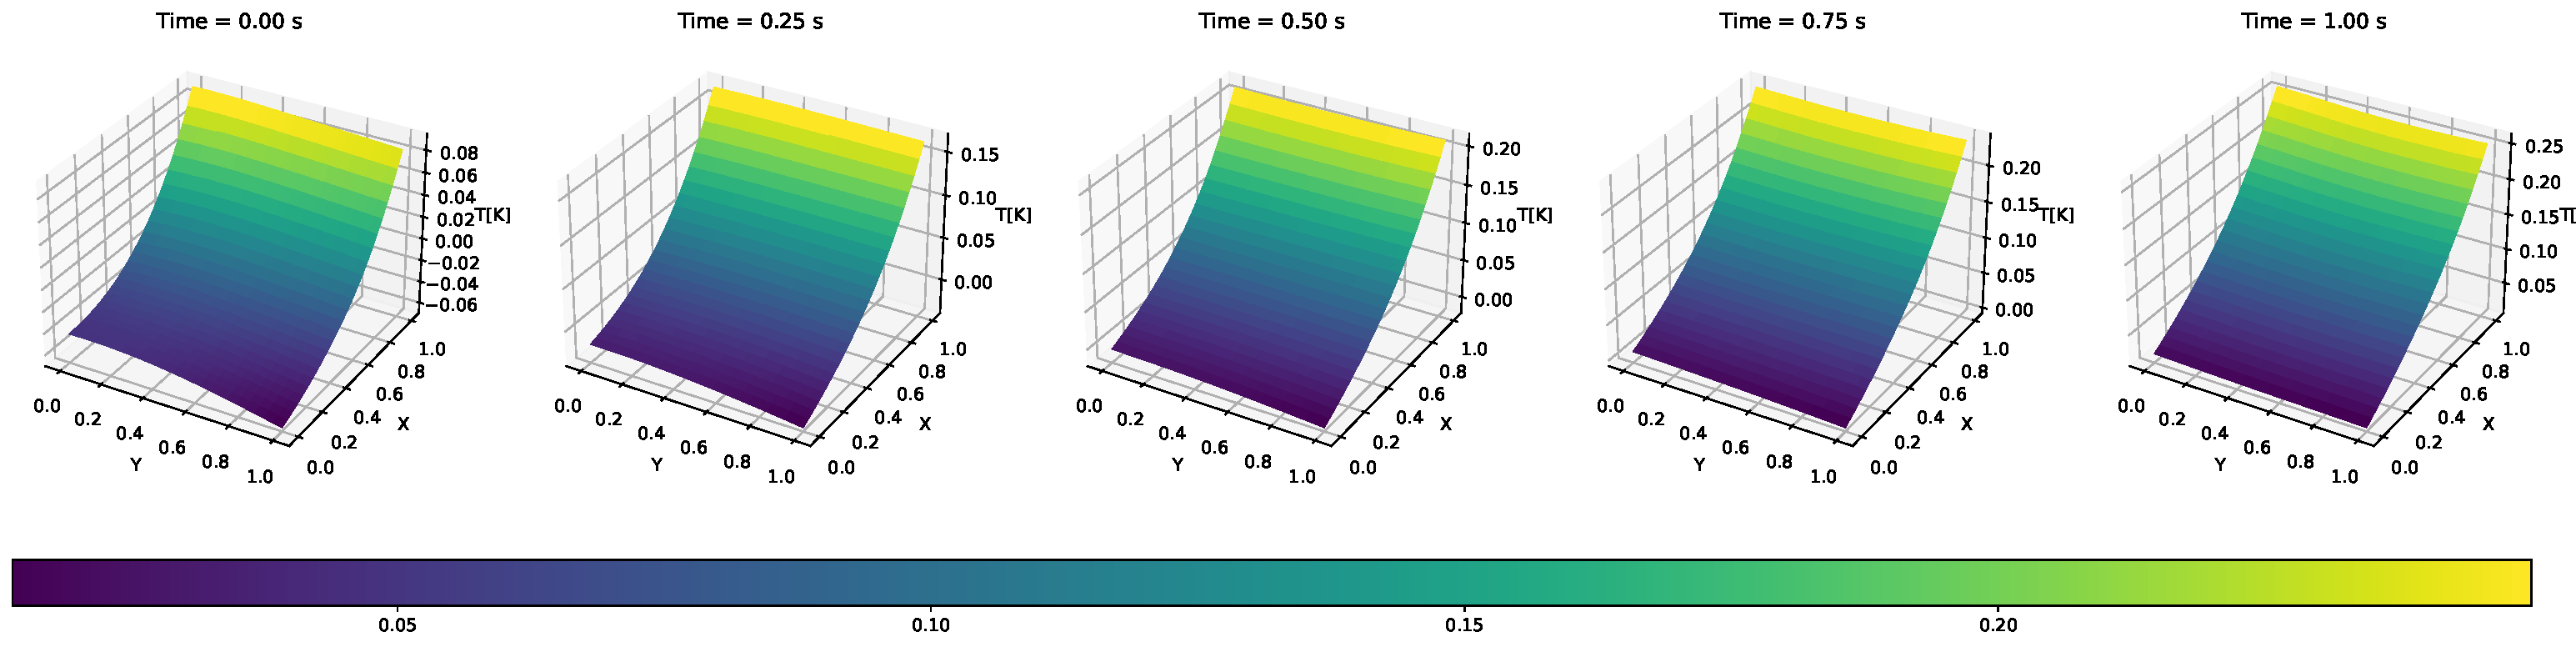
\includegraphics[keepaspectratio]{predicciones_files/figure-pdf/fig-my_results-output-1.pdf}}

}

\caption{\label{fig-my_results}Predicciones de la red neuronal a
distintos tiempos.}

\end{figure}%

\begin{figure}

\centering{

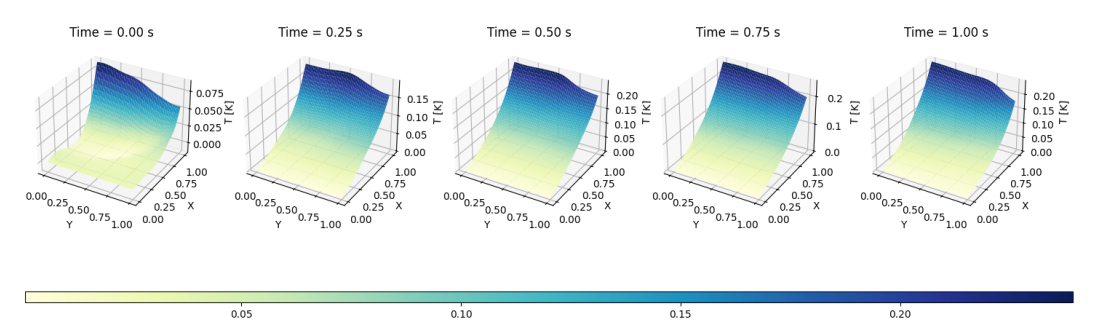
\includegraphics[width=7.8125in,height=\textheight,keepaspectratio]{images/results_paper.png}

}

\caption{\label{fig-results_fnn}Resultados reportados por Alessio Borgi
(\citeproc{ref-medical_rep}{2023}) en el caso 2D.}

\end{figure}%

\bookmarksetup{startatroot}

\chapter*{Referencias}\label{referencias}
\addcontentsline{toc}{chapter}{Referencias}

\markboth{Referencias}{Referencias}

\phantomsection\label{refs}
\begin{CSLReferences}{1}{0}
\bibitem[\citeproctext]{ref-medical_rep}
Alessio Borgi, Alessandro De Luca, Eugenio Bugli. 2023. {«{BioHeat
PINNs: Temperature Estimation with Bio-Heat Equation using
Physics-Informed Neural Networks}»}.
\url{https://github.com/alessioborgi/BioHeat_PINNs/tree/main?tab=readme-ov-file\#bioheat-pinns-temperature-estimation-with-bio-heat-equation-using-physics-informed-neural-networks}.

\bibitem[\citeproctext]{ref-blechs2021}
Blechschmidt, Jan, y Oliver G. Ernst. 2021. {«Three ways to solve
partial differential equations with neural networks---A review»}.
\emph{GAMM-Mitteilungen} 44 (2): e202100006.
\url{https://doi.org/10.1002/gamm.202100006}.

\bibitem[\citeproctext]{ref-dutta2018}
Dutta, Abhijit, y Gopal Rangarajan. 2018. {«Diffusion in pharmaceutical
systems: modelling and applications»}. \emph{Journal of Pharmacy and
Pharmacology} 70 (5): 581-98. \url{https://doi.org/10.1111/jphp.12885}.

\bibitem[\citeproctext]{ref-nci2021}
Instituto Nacional del Cáncer. 2021. {«{¿Qué es el cáncer?}»}
\url{https://www.cancer.gov/espanol/cancer/naturaleza/que-es}.

\bibitem[\citeproctext]{ref-karniadakis2021}
Karniadakis, George Em, Ioannis G. Kevrekidis, Lu Lu, Paris Perdikaris,
Sifan Wang, y Liu Yang. 2021. {«Physics-informed machine learning»}.
\emph{Nature Reviews Physics} 3 (6): 422-40.
\url{https://doi.org/10.1038/s42254-021-00314-5}.

\bibitem[\citeproctext]{ref-kumar2024deeponet}
Kumar, Varun, Somdatta Goswami, Katiana Kontolati, Michael D. Shields, y
George Em Karniadakis. 2024. {«Synergistic Learning with Multi-Task
DeepONet for Efficient PDE Problem Solving»}. \emph{arXiv preprint
arXiv:2408.02198}. \url{https://arxiv.org/abs/2408.02198}.

\bibitem[\citeproctext]{ref-lu2021deeponet}
Lu, Lu, Pengzhan Jin, Guofei Pang, Zhongqiang Zhang, y George Em
Karniadakis. 2021. {«Learning nonlinear operators via DeepONet based on
the universal approximation theorem of operators»}. \emph{Nature Machine
Intelligence} 3 (3): 218-29.
\url{https://doi.org/10.1038/s42256-021-00302-5}.

\bibitem[\citeproctext]{ref-deepxde}
Lu, Lu, Xuhui Meng, Zhiping Mao, y George Em Karniadakis. 2021.
{«{DeepXDE}: A deep learning library for solving differential
equations»}. \emph{SIAM Review} 63 (1): 208-28.
\url{https://doi.org/10.1137/19M1274067}.

\bibitem[\citeproctext]{ref-hyperthermia}
National Cancer Institute. 2021. {«{Hyperthermia to Treat Cancer}»}.
\url{https://www.cancer.gov/about-cancer/treatment/types/hyperthermia}.

\bibitem[\citeproctext]{ref-omscancer}
Organización Mundial de la Salud. 2022. {«{Cáncer}»}.
\url{https://www.who.int/es/news-room/fact-sheets/detail/cancer}.

\bibitem[\citeproctext]{ref-pennes1948}
Pennes, H. H. 1948. {«Analysis of Tissue and Arterial Blood Temperatures
in the Resting Human Forearm»}. \emph{Journal of Applied Physiology} 1
(2): 93-122. \url{https://doi.org/10.1152/jappl.1948.1.2.93}.

\bibitem[\citeproctext]{ref-quintero2017}
Quintero, Luis A., Mauricio Peñuela, Armando Zambrano, y Edwin
Rodríguez. 2017. {«Optimización del proceso de preparación de soluciones
madre de antibióticos en un servicio farmacéutico hospitalario»}.
\emph{Revista Cubana de Farmacia} 50 (2): 448-65.
\url{https://www.medigraphic.com/cgi-bin/new/resumen.cgi?IDARTICULO=75483}.

\bibitem[\citeproctext]{ref-yang2014}
Yang, Lihong, Xin Wu, Qian Wan, Jian Kong, Rui Liu, y Xiaoxi Liu. 2014.
{«Pharmaceutical preparation of antibiotics: a review on formulation and
technique»}. \emph{Asian Journal of Pharmaceutical Sciences} 9 (3):
145-53. \url{https://doi.org/10.1016/j.ajps.2014.04.001}.

\end{CSLReferences}




\end{document}
